% !TeX root = sigui-manual.tex
\chapter{User interface}
\section{Updater configuration}
When you open SigUI the \emph{Updater configuration} tab is open, see \prettyref{fig:tab1}.
\begin{figure}[htb]
\centering
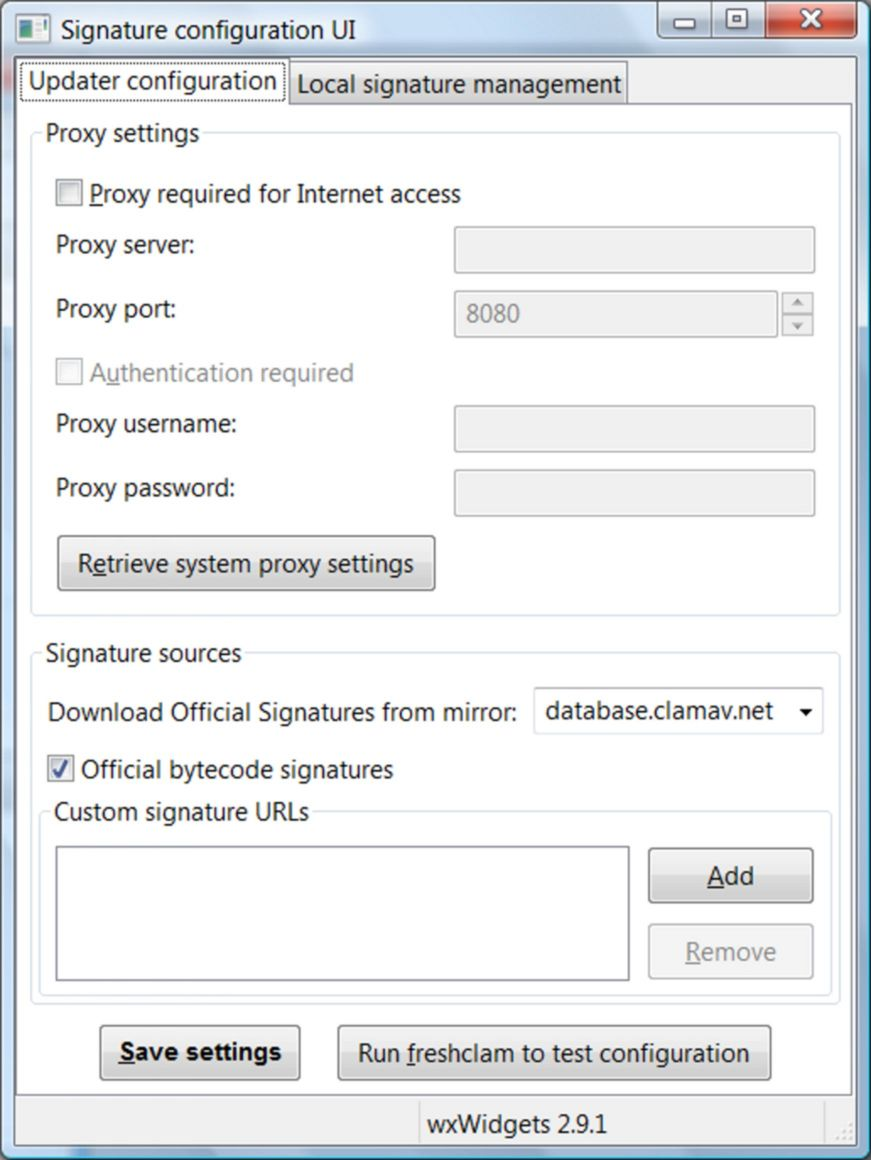
\includegraphics{sigui_tab1.jpg}
\caption{Updater configuration}
\label{fig:tab1}
\end{figure}

It has 2 sections:
\subsection{Proxy settings}
If \emph{Proxy required for Internet access} is not ticked, then \gls{freshclam} will connect directly to the internet.

If it is ticked, then the \emph{server} and \emph{port} fields, and \emph{Authentication required} checkbox will be enabled.

If the \emph{Authentication required} checkbox is ticked the \emph{username} and \emph{password} fields will be enabled too.

The \emph{Retrieve system proxy settings} will attempt to retrieve the proxy settings from Internet Explorer, and fill the above fields.

See \prettyref{sec:proxysettings} for an example.

\subsection{Signature sources}
Here you can configure what databases will \gls{freshclam} automatically download.

\emph{Download Official Signatures from mirror} allows you to choose the \gls{mirror} that \gls{freshclam} will use to download the virus databases. You can either enter a custom hostname, or select one from the list (preferably the one that matches your countrycode).
See \prettyref{sec:mirror} for an example.

\emph{Official bytecode signatures} is by default enabled. If you want to disable it, untick it. But you must be aware that you will miss some detections, or even bugfixes.

\emph{Custom signature URLs} is a list of custom URLs that \gls{freshclam} will download and install as new virus signature databases.
You can use the \emph{Add} and \emph{Remove} buttons to manage the list. The list accepts \verb+http://+ URLs, or \glspl{UNC path}.
See \prettyref{sec:customsigs} for detailed examples.

\subsection{Saving configuration and testing}
Pressing the \emph{Save settings} will validate all the fields on this tab, and save the settings to \gls{freshclam.conf}. If there is anything wrong an error message will be shown.

Pressing the \emph{Run freshclam to test configuration} will test whether the new \gls{freshclam.conf} works as expected. If this results in error you should fix it, otherwise your custom databases won't be used.\footnote{The official ones should still be downloaded correctly even in case of errors, unless freshclam.conf is very broken}

\section{Local signature management}
This tab allows you to manage the signatures installed in the database directory, see \prettyref{fig:tab2}.

\begin{figure}[htb]
\centering
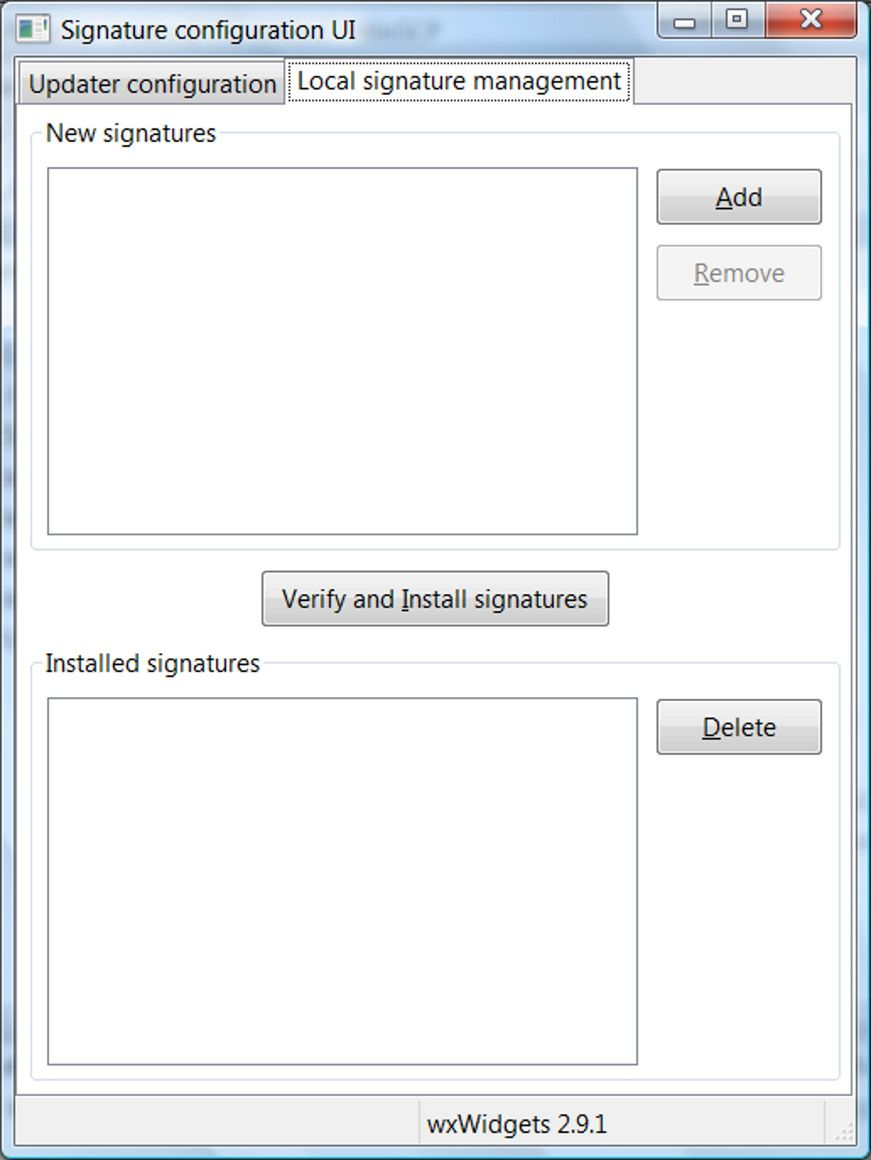
\includegraphics{sigui_tab2.jpg}
\caption{Local signature management}
\label{fig:tab2}
\end{figure}

There upper section, \emph{New signatures} shows the signatures you are about to install,
and the bottom section, \emph{Installed signatures} shows the already installed signatures.
You can manage the top list using the \emph{Add} and \emph{Remove} button (Add launches a standard \emph{Open file} dialog).

The bottom list is managed by SigUI and \gls{freshclam}. You can press \emph{Verify and Install signatures} to validate and copy the signatures from the list above to the one below.
Signatures are only copied after they have been verified as valid, an error is shown for malformed signatures. See \prettyref{sec:custommanual} for an example.

The \emph{Delete} button will delete the actual signatures files from disk, it should be used only if you know what you are doing (a confirmation message is shown prior to delete of course).

\section{Run freshclam to test configuration}
\label{sec:runfreshclam}

Pressing this button will launch \gls{freshclam}, and opens a window to show its output, see \prettyref{fig:freshclamout}.

\begin{wrapfigure}{r}{0.5\textwidth}
\centering
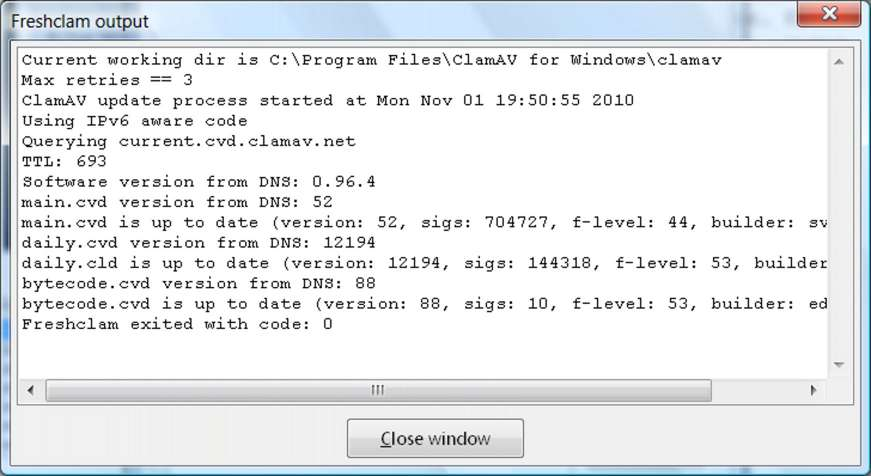
\includegraphics{sigui_run.jpg}
\caption{SigUI: Freshclam output window}
\label{fig:freshclamout}
\end{wrapfigure}

The output shows the progress of the update, and any error messages from \gls{freshclam}.
It is recommended that once you change \gls{freshclam.conf}, by clicking \emph{Save settings}, to test it by clicking on \emph{Run freshclam to test configuration}.

The window has a button to forcefully terminate \gls{freshclam}, but this should only be used if for some reason it hangs. Note that by default the timeout for connecting to a remote server is 30 seconds, so you should wait at least 30 seconds before terminating it.

Once \gls{freshclam} finishes the button changes to a \emph{Close window} button, that can be safely pressed to dismiss the window.

\section{Custom URLs}
\label{sec:ui_urladd}
The \emph{Custom signature URLs} section on the \emph{Updater configuration}
page allows you to add custom URLs.

\Gls{freshclam} will automatically download these each time it updates the official signatures (usually once an hour).
If your webserver supports \verb+If-Modified-Since+ headers, it will only
download the new database if it is newer than the already installed one.

Digital signatures  are checked only for \gls{CVD} signatures\footnote{because they are the only ones that contain such signatures}.
Freshclam automatically tests all signatures (for syntactic correctness) after downloading, but
before installing them. If a signature file is malformed it is not installed and
an error is logged.

Usage:
\begin{itemize}
\item Click Add to add a new URL, press OK when done
\item If the URL is not in the correct format, an error message is shown.
Correct the URL and press OK again.
\item The new URL shows up in the \emph{Custom signature URLs} section
\item Add as many URLs as needed
\item You can remove an URL by clicking the \emph{Remove} button.
\textbf{WARNING}: If the database was already downloaded it won't remove the downloaded signature file from the disk.
See \prettyref{sec:localremove} on how to do that.
\item Check that you entered the correct URLs.
\item Click \emph{Save settings}.
\item Click \emph{Run freshclam to test configuration} to make sure freshclam is
able to correctly download the signatures. Freshclam will only install
signatures that are in the syntactically correct.
See \prettyref{sec:runfreshclam}
\end{itemize}

Note that the downloaded signature files will all be placed in the same directory. Hence you must make sure you don't have two URLs that, when downloaded, have the same filename.
The UI will warn you if you try to do that. \footnote{the two URLs with same filenames will just keep overwriting the same file}.
\section{Update now}
\label{sec:updatenow}
Any changes you make to \gls{freshclam.conf} and the databases won't take effect immediately.
They will take effect the next time the signatures are updated (usually once an hour).
To reload the signatures immediately open the \CW user interface from the tray (or desktop icon), and click on \emph{Update Now}. 
Once the database is updated, it will be reloaded as soon as the system is idle.